\documentclass[a4paper,11pt]{article}
\usepackage[margin=3cm]{geometry}
\usepackage{float}
\usepackage[T1]{fontenc}
\usepackage{inputenc}
\usepackage{amsfonts}
\usepackage{graphicx}
\usepackage{bm}
\usepackage{varioref}
\usepackage[english]{babel}
\usepackage{hyperref}
\usepackage{tikz}
\usetikzlibrary{arrows,decorations.pathmorphing,backgrounds,positioning,fit,petri}
\usepackage{enumitem}
\usepackage{newclude}
\newcommand{\field} [1] {\mathbb{#1}}
\newcommand{\mil}{Musik I Lejet }
\begin{document}

\begin{titlepage}
\centering \parindent=0pt
\newcommand{\HRule}{\rule{\textwidth}{1mm}}
\vspace*{\stretch{1}} \HRule\\[1cm]\Huge\bfseries
MIL Project\\\emph{Musik i Lejet}\\[0.7cm]
\HRule\\[4cm]  \large  Jägerne
\\Jacob Stenum Czepluch (jstc@itu.dk), \\

\vspace*{\stretch{2}} \normalsize %
\thispagestyle{empty}
\begin{flushleft}
BFOP \\
Bachelor in Software Development\\
IT-University of Copenhagen\\
December 15, 2013 \end{flushleft}
\end{titlepage}

\tableofcontents
\pagebreak

\pagebreak
\section{LOL}
pops


%!TEX root = /Users/Abj/git/MiL/report/report.tex
\part{Summary}

\section{About}
Introduction... 

How can the board delegate responsibility of the planning and execution of Musik i Lejet to the management? 

Measurements:
Topics on board meeting minutes, identified by the board as topics subject to management, should be reduced by x%


\section{List of activities}
We have created a list to give an overview over which kind of activities we have conducted doing the project and when we did them. The list can be found in appendix XX
\begin{center}
\begin{table}
    \begin{tabular}{|p{3cm}|p{3cm}|p{3cm}|p{6cm}|}
    \hline
    Date & Type of activity & Participants & Comments \\
    29 - 09 - 13 & (non-formal?) Interview & MiL: Andreas Workgroup: All & The workgroup presented the scope(?) of the course and got an initial idea of the organization and the role that Andreas have in MiL.  \\
    31 - 10 - 13 & (formal?) interview  & MiL: Christian og Stakkeman &  .......  \\
    \end{tabular}
\end{table}
\end{center}
\section{Figure of organization}
First draft of organizational diagram. Needs to be confirmed by MiL
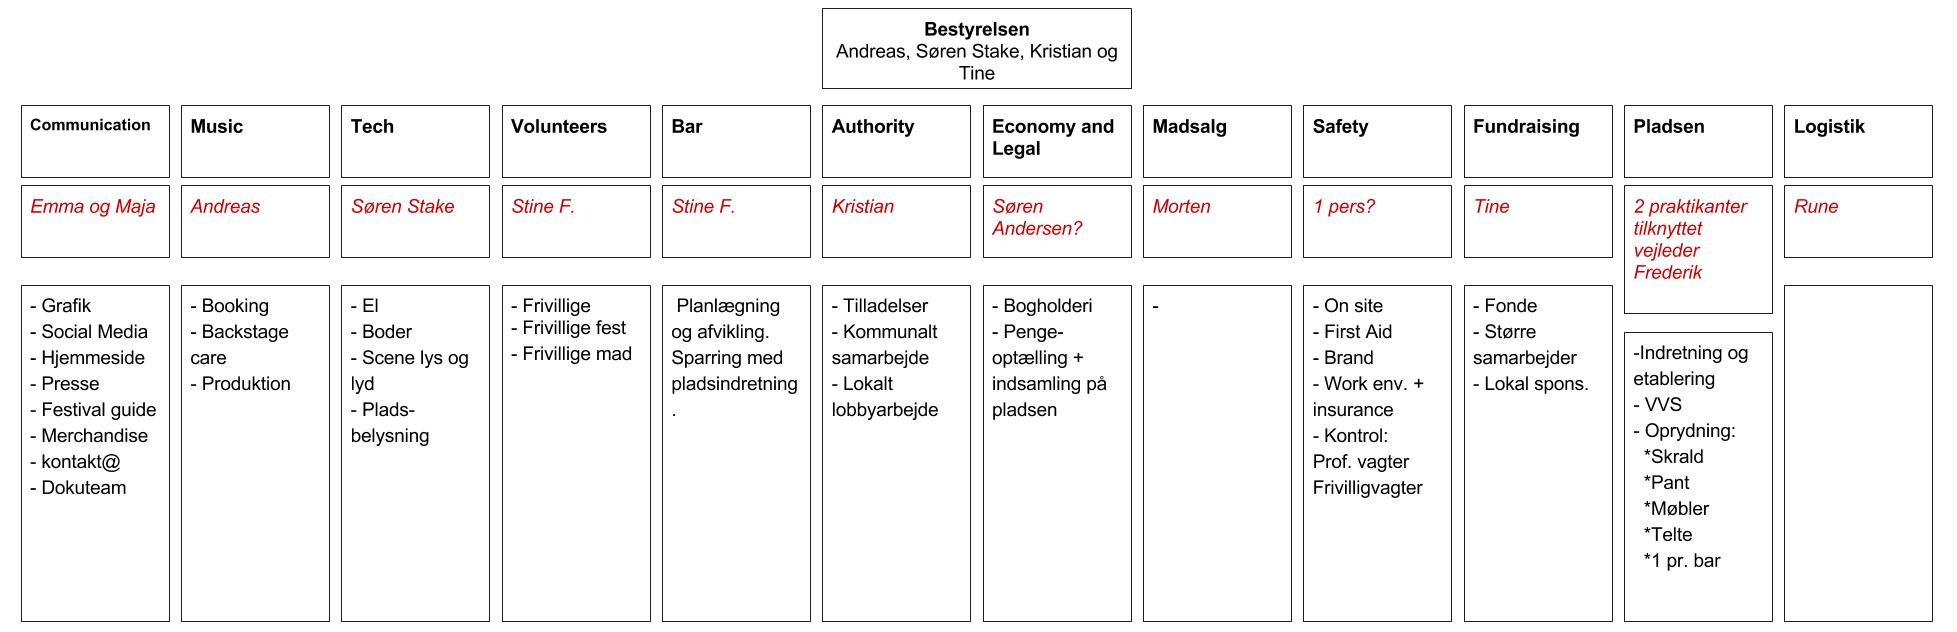
\includegraphics[scale=0.3, angle=90]{Pictures/MIL_Organisational_chart-Ledelsen.jpg}
\section{Business and IT scope}
For this project the workgroup have chosen to focus on the managing part and more specific the board of Musik I lejet. We will also look at how the internal communication is shared between all members and what kind of work processes is in play when planning the festival. \\
Must of the communication is done at Musik i Lejet's Podio site and therefore we will direct our attention and observations towards that platform. Since this projects is done before the actual festival takes place, we will primarily focus on IT used before the festival, which to our belief, is only Podio.  

\part{In-line Analysis}

\section{Business Strategy}
The main objective of Musik i Lejet is to provide a cultural offer in the local community of Tisvildeleje, both as an offer to the local populous, and also to attract business to the community. This is achieved by a non-profit, cost driven business model, that relies heavily on volunteer work, grant money and private sponsorship. Cultural and economic value is generated by offering musical entertainment for a variety of customer segments, such as music enthusiasts, families with children and customers interested in attending parties.
\\ \\
Keeping a well defined and contemporary musical profile is essential for Musik i Lejet to fulfill both its cultural objectives, and to make the festival competitive with other festivals of the same size, addressing the same customer segments. Moreover, diversity within the festivals audience is of huge importance to Musik i Lejet. This is in part achieved by offering a wide selection of music in many different genres, but also by keeping ticket prices low, and providing free admission for children and the elderly.
\\ \\
The main challenges for Musik i Lejet include maintaining relationships with and interest from sponsors and cultural foundations, securing the necessary number of volunteer workers, coordinating the efforts of the 20-30 people who, without a physical and centralized work space, arrange the festival in their spare time, and obtaining contracts with contemporary and popular performing artists to an affordable price.

\section{Environment}
When studying MiL it is of importance to view it in the relative perspective of its surroundings to be able to determine strengths/weaknesses as well as relations, ultimately to support potential solutions. In this case we deal with the remaining forces of danish music festivals.
\\  \\
The industry of danish music festivals is a healthy and growing market showing indications of trends towards an increasing appreciation of larger live events. Many festivals exists as of today, but differentiate significantly in vision, identity, and size. This means that when considering the market, competition to MiL can not be inferred if they do not target the same customer segments. Due to MiLs price and target segments, opposing threats are few in numbers, e.g. Wonderfestiwall and trailerpark festival. This compitition fails to compete with MiL by due to the significent difference in ticket price.
\\  \\
Stable relationships with providers and stakeholders are of big part of what makes MiL possible, and are therefore an important aspect to maintain and care. Due to success throughout MiLs past years of events can provide stability as an organisation through factors such as: sold out events, positive publicity and continous increase in revenue. With this MiL has established quality cooperation agreements providing security and avoiding risk at depencies.
\\  \\
A potential risk occuring as a product of MiLs increasing success is the organisations capability of scaling its internal resources to match a larger event while maintaining the same value offer - This in view of the environment MiL lacks experience due to its relative young age. Failing to being able to cope with expansion could result in increased ticket prices. This would remove MiLs advantage, enabling competition to become competition


\section{Work Domains}
\label{sec:work_domains}
\subsection{The board}
\label{sub:the_board}
The main responsibility of the board is to make all major decisions regarding the execution of the
festival. They are also responsible for all strategic decisions and they handle the booking of
some of the big artists and the approval of expensive contracts and deals that the teams make.

\subsection{The team leaders}
\label{sub:team_leaders}
The team leaders each have an area of responsibility which results in a team leader being
responsible and the leader of a team of volunteers that focus on a specific area of the festival
planning. As seen in the \ref{sub:organisation} there are 12 independent teams. The most important
role of a team leader is to communicate with the other team leaders and give feed back to the board
regarding the status of the team's current tasks. Team leaders meeting are held once every ?????,
where the team leaders give status updates to each other and discuss inter team problems and
deadlines.

\subsection{The team members}
\label{sub:team_members}
A team member is simply a volunteer that help out with the planning of the festival, and not only
the execution. As a member of a team you will be given different tasks accomplish depending on which
team you are in. If you are in the bar team, a task could be to make sure that offers for bar tents
have been obtained before a certain deadline. 


%!TEX root = /Users/Abj/git/MiL/report/report.tex
\part{In-depth Analysis}

\section{Organizational setup, key players and KPI's}
\subsection{Organizational setup}
\subsubsection{Structural Change}
Before the project period was started the organization initiated a structural change. This influenced the board, but mostly the planning group, since this was expanded from X to Y members. This change was conducted in order to move and spread the knowledge and responsibility from the board across the organization, by delegating responsibility to leaders in different planning teams(interview kilde).

\subsection{Key Players}
Several types of key players can be identified in the organisation. Before the structural change, the level of key player, was determined by each persons experience with planning of Mil. Naturally, most of the key players was also part of the board.\\
With the newly structural change, these players are made responsible for a team, which enforces two things. Firstly, a lot of the planning are moved away from the board. Second, when delegating a person as a leader for a team, the knowledge for this particular area of planning is more assigned to a role in a team instead of a specific person. The consequences of this change, is that more key players can be identified, which creates more dependencies between the different area of planning, since more people are involved(kilde på at flere mennesker skaber mere afhængigheder).\\
Thereby, the current most interest key players are the leaders of each teams, which the stakeholder analysis in appendix xx suppports.\\
Bilag: STAKEHOLDER ANALYSIS??????\\

\subsection{Key Performance Indicators}
Top level KPI -> deadlines eksempel\\

Bilag:\\
Top level KPI's\\
finanical Stability\\
	- Ticket price\\
	- keeping budget\\
Podio\\
- 24 hour rule\\

KPI's: Ticket price, financial stability, keeping the budgets, 24 hour rule of podio\\

At this point of the project we identified a number of KPI's and we will use this section to underline some of the aspects according to these.\\
As described in appendix xx MiL has several top level KPI's which is crucial in respect to customer satisfaction and the overall sale during the festival(kilde?). 

\section{Current work practices}
This section will describe some of the work there is, when working in the planning group of Mil. Before going in to the actual descriptions, we do however need to mention, that observing work practices in an organization as this, is not a trivial task. We have observed the work practices in the form of interviews and an observation at the General Assembly, which hardly can be formulated as actual practices, but more as a mean to work. However, we have found several things, which we believe can be used as documentation for the practices. \\
At the General Assembly a suggestion from the board was raised, about all members being charged a fee for being part of MiL. The board explained that this was more a matter of regulation of a union, and to get some financial advantages, than a need for payment. The non-board(?) members raised some concerns regarding this issue, as stated in appendix xx. Surprisingly, even though the non-board members raised strongly concerns, the board decided to proceed with the suggestion, without a voting about it. \\
The board also included a short presentation of Podio at the General Assembly. As stated in appendix xx the board wants to have all internal communication in the planning group at Podio. This was clearly a new tool for some of the leaders, which was stated in the form of different questions(kilde?). Most of the presentation was about the different subpages at Podio and how to create things like events and tasks. This gave some insight what Podio is cable of, but no introduction was given about when a task was done nor when a task should be created for another member (better examples?).\\

During the interview with Stine F the project group made her participate in a 'process'-game. Here the interviewers asked her to explain the task of booking volunteers for the festival. The result of this game can be seen in appendix xx. In our opinion it clearly shows that a lot can be done in termns of deadlines for bookings of volunteers and also the way its done.

- Stemning og struktur på General Forsamling (blandt andet forslag om kontigent blev ikke besluttet)\\
- Podio (manglende af done og done-done) og noget andet?\\
- Problem med høj overpris af hegn\\
- Beskrivelse af process spil

\subsection{Goals, problems, and needs}
In this section we will summarize the goals, problems, and needs that the
in-depth phase analysis has lead us to.

\subsubsection{Goals}
It is clear to us, according to \ref{interview source} that it is a goal for \mil to cut down
the amount of missed deadlines.
\\
Some parts of the board \ref{Kristian source} sees it as a goal that the
budget is not only kept, but that the offers collected on expensive things, are
also the best offers.
\\
There is also a certain desire \ref{Learn podio reference} that everyone knows
how to use Podio, since the board demands that Podio is the single point of
communication for \mil.

\subsubsection{Problems}
According to our analysis \ref{source}, some problems are made clear. \\
              \begin{itemize}
    \item It is neither clearly stated when different tasks are due to
    internally in the different groups nor between the working groups.
    \item People leaves out some information on Podio, because they do not know
    how to add it properly.
    \item There is no single place on Podio where all important deadlines are
    put.
    \item There is no clear guidelines for when a task is done.
    \item (Add more if any...)
\end{itemize}

\subsubsection{Needs}
After several interviews with different people from \mil, it is clear to us that
there are some common needs.
\begin{itemize}
    \item According to \ref{source} there is a need for a system that makes it
    clear to everyone which deadlines are due to when.
    \item Guidelines describing when a task is done are also needed
    \ref{source}.
    \item A common understanding and knowledge of how the basics of how Podio
    works, assuring that everyone is able to document the progress of their work
    and tasks is also needed \ref{source}.
\end{itemize}


\subsection{Ideas for solutions}
In this section we will discuss some of the ideas we have for technical
solutions to help ease the organisational restructuring of \mil.

\subsubsection{Podio workshop}
It has come to our attention when attending \ref{General Assembly Appendix} that
a lot of the volunteers have very little knowledge of how Podio works. Due to
this, one of our suggestions is to make a Podio workshop that teaches the basics
of Podio the way the board of \mil has in mind that is should be used.

\subsubsection{Podio tutorial}
In addition to this, a tutorial made in Podio that uses the features of Podio to
teach how Podio works, is also a solution that we believe to be very useful
\ref{reference to something about how good learning hands on is} in the process
of learning how to use Podio.

\subsubsection{Podio App}
Since it is a goal \ref{source to this} that all communication should take place
on Podio, we would like to make a Podio app that allows the user to make tasks
and dependencies for each area of responsibility in the different groups.

\subsubsection{Done and done done}
There is a concern amongst some of the board members \ref{source from meeting
with Andreas} that since each responsibility group now have their own budget to
administer they will not necessarily use energy to find the best offers on the
market. Our solution proposition is to make a rule that when a person gets the
responsibility to find offers on eg the fence surrounding the festival area, the
person has to collect three offers and the rest of the responsibility group now
has to decide which one is best. The task to find an offer on the fence is now
done, but it is not marked as done done before the contract is signed.

\subsubsection{Wiki}
We have also found out that it is a pain \ref{source to interview} to have a
common place to share knowledge between the groups. A possible solution to this
is to make an app that makes it really easy to add knowledge to a shared wiki
through Podio.


%!TEX root = /Users/Abj/git/MiL/report/report.tex
\part{Innovation}
%As the previous sections of the \texttt{In-depth phase} in part \ref{prt:in_depth_analysis},
%especially in section \ref{sub:goprne}, has shown,
%the organisation has room for optimisation and improvements. Based on the \ref{sub:ideas} that we
%have developed and the fact that the organisation wants to continue using Podio, we have chosen two that we believe will bring the most benefits to the organisation.
%We will in the following analyse both the solutions, and try to determine which will be the best or
%if a third solution will emerge from this analysis. A short description of the ideas in focus
%follows:


%1. Work processes for Podio\\
%In the previous the Diagnostic Map in section xx revealed several problem and related causes found in the organization. In 5b its said that the cause of this problem, is that their is too much off topic discussion and also that no real difference between pure informational topics and topics for discussions are in place within the organizational use of Podio. As Stine F also points out in 1a, the organization faces a problem about sharing of knowledge, since this is not documented properly on Podio.\\

%This solution proposal will attempt to structure work processes when using Podio and make guidelines for the information posted at Podio. This proposal will therefore be  directed at the use of Podio, with respect to the mentioned things in the above, and will keep to the organizations strategy about using Podio as their primary IT solution. 

%2. Podio App
%This solution consists of the development of a Podio application \footnote{https://developers.podio.com/doc/app-store}.
%The application will be used to create, store, and visualise tasks in- and externally in the teams.
%Thus, hopefully, making it very transparent which tasks are due to when.\\

\section{WORK PROCESSES}
\subsection{Visions for change}
The visions for this solution proposal is a bit different, than what is normally suggested as a
solution, since this does not contain an actual implementation of a new IT solution, but rather a
change in the way the current system is used by the organisation.
Podio is very customisable and offers per default the possibility to create your own applications
suited for your needs. This solution will however focus solely on changing the way the organisation
is using their current available tools and work practices in Podio.


%The overall vision for the change, can be divided in to these subsections:
\subsubsection{Information at Podio}
As mentioned earlier, and seen on Podio, a lot information is non-relevant for the actual planning and should therefore be elsewhere. Based on the analysis, we believe that the reason for this non-relevant information is on Podio is due to the relaxed working environment shared by the members and also the lack of formal guidelines for what kind of information should be posted on Podio, by whom and when.\\ 
We suggest that the board makes a formal description of these, by categorizing them after importance.
This will impact every member of the planning group and board, since an equal amount of non-relevant information seems to be posted between all members. \\

Make scenario for how this new work practice will be for the persons impacted by it(p191)
  
\subsubsection{Sharing of knowledge}
With an organization structured and based highly upon volunteers like Musik I Lejet, there is always a risk of people leaving the organization with short notice and taking valuable information and knowledge with them. Since this risk is hard to limit, the solution proposal will try to embrace the knowledge that the members poses and expose this at relevant places on Podio, for others to use. The challenge with this, is to find the persons holding the knowledge and exploring it, since some of it may be tacit(use different levels of knowledge theory). A challenge is also to document this is a right way, so it can be reused at a later point and saving in a place on Podio where others will be able to find it.\\
The team leaders is probably the target for this part of the solution, since most of these a highly experienced and has a good feel about the different areas of the organization.\\

Make scenario for how this new work practice will be for the persons impacted by it(p191)

\subsubsection{Sharing of decisions and agreements}
Throughout the analysis phase, it has been pointed out that members of the organization find it hard to find out what decisions and agreements there have been made and where it is documented. Reasons for this is the causes mentioned in 2b and 4b in the Diagnostic Map in appendix xx. MORE STUFF HERE\\ 
Make scenario for how this new work practice will be for the persons impacted by it(p191)

\subsection{Technology}
Since this solution is based on the IT system that the organisation already uses, there is no point
in explaining the technology too much. A short summary of Podio can be found in the glossary in
section \ref{sec:glossary} and \ref{sec:technology}.

\subsection{Work organization}
As mentioned above, this solution, does not need an implementation of a new IT system. It does how
ever consist of changes to the work organisations of the organisation. 
We have concluded in section \ref{podio bloat source} that a lot of the information and
communication on Podio is irrelevant to the planning of the festival. It seems that a good solution
to this, would be to make some guidelines in cooperation with the board that states what kind of
communication should take place on Podio and where it should take place. If most of the irrelevant
comments and posts dissapeared, the change of overlooking important information and deadlines
decreases. 
* Frivillig organisation, de gør det også for at have det sjovt
* 

\subsection{Qualification needs}

\subsection{Advantages and disadvantages}

\subsection{Finances}

\subsubsection{Roll out}

\subsubsection{Training}
Forslag: Experts and normal users
\subsubsection{Data conversion}
Converting all the existing Podio data to be alligned with the new formal structure for information, knowledge and decisions...

\subsection{Implementation strategy}
The must effective way this solution can be implemented in the organization will be as a pilot project, where selected members of the organization will be trained in how to use the formal ... 



\section{Podio extension}
\subsection{Visions for change}
\label{visions_for_change}
This solution is at its heart an interactive visualization of tasks and task dependencies across arranger teams. Tasks are communicated between arranger teams with the already present infrastructure present in Podio. The task window however, is extended with the following functionality and data:
\begin{itemize}
    \item Tasks can include subtasks. Subtasks are added to a task by pressing the "Add Subtask" button. When teams assign tasks to other teams, the receiving team may choose to define subtasks, that need to be completed before the assigned task can be completed. Subtasks can either be already existing tasks, or new tasks.
    \item Tasks include a "Done" description, in which the sender of the task may include a short description of when the task is considered to be done.
    \item Tasks are done when the receiving team presses the "Done" button under a task.
\end{itemize}
The data and functionality described above makes it possible to create a task map. The task map displays all active tasks in the system. A task is active if any of its subtasks are incomplete, or if it is itself a subtask to a task that is incomplete. Tasks are displayed graphically, with dependencies between them drawn as an directed arrow between them. Clicking a task will take the user to the task on Podio, where a detailed view of the task can be found. 
\\ \\
This solution will give arrangers an overview of deadlines, tasks associated with deadlines and dependencies between them across arranger teams, as to address problems discussed in (ref diagnostic map). By extracting deadline information and placing it collectively in the task map, confusion about where to find information about deadlines is reduced.


\subsection{Technology}
\label{sub:technology}
The solution uses the built in functionality of Podio to build custom Podio apps to create the needed modifications to Podio tasks. The task map is drawn on a webpage outside of the Podio domain, using the Podio REST API.

\subsubsection{IT systems and IT platform}
The solution is primarily dependent on the existing Podio platform. It is necessary that Podio maintains the possibility of defining custom apps and accessing Podio data through the REST API.

\subsubsection{User interfaces}
On Podio, the interface is built using the existing Podio app builder tools. The task map is displayed by some Web UI technology. Tasks are shown as nodes, and dependencies between them are shown as directed arrows. Task completion status is indicated graphically by color. (ref til mock up)

\subsection{Work organisation}
\label{sub:work_organisation}
Arrangers and team leaders will have to change their work-flow with creating tasks, to comply with the format described in section \ref{visions_for_change}. An introduction to using the task map must also be created. Some teams already use tasks (ref til podio analyse), and others do not. The teams that are not familiar with tasks will have to be introduced to them, and some encouragement and reinforcement is likely to be necessary.

\subsection{Qualification needs}
\label{sub:qualification_needs}
The solution depends on arrangers and team leaders using Podio correctly. This means that arrangers and team leaders must know how to use Podio.

\subsection{Advantages and disadvantages}
\label{sec:advantages_disadvantages}
\begin{center}
    \begin{tabular}{ | p{7cm} | p{7cm} |}
    \hline
    \textbf{Advantages} & \textbf{Disadvantages}  \\ \hline
     Raises awareness of deadlines and dependencies between teams & Risk of arrangers not using the system\\ \hline
     Makes information about deadlines easier to find & Time must be invested in teaching arrangers how to and when to create tasks\\ \hline
     Integrated with a system that is already known and used by arrangers and team leaders & Solution is dependent on Podio maintaining custom app possibilities and a Web service interface \\ \hline
    \hline
    \end{tabular}
\end{center}


\subsection{Finances}

\subsection{Implementation strategy}
The pilot project strategy is recommended for this solution. Potential short comings and problems can be corrected before trying it with the whole organization. The bar team, fetival site team and volunteer team are good candidates for pilot teams, as significant dependencies exist between them (ref til stine interview eller flowchart).

A possible challege when implementing the strategy is motivating arrangers and team leaders to assign tasks on Podio, instead of sending messages or posting on walls of other groups etc. One strategy is to demonstrate the value of the task map, and how the usefulness of this tool is increased for everyone, when more arrangers use the task feature of podio.


%\include{Appendix/...}

%\pagebreak
%\include*{FOLDERNAME/FILENAME}


\end{document}
